\documentclass[11pt]{article}

%\usepackage{palatino}

\usepackage[utf8]{inputenc}

\usepackage[sfdefault, scaled=.85]{roboto}
\usepackage[T1]{fontenc}
\usepackage{textcomp}
\usepackage{amsmath,amsthm}
\usepackage[cmintegrals]{newtxsf}
\usepackage[italic]{mathastext}
\usepackage[spanish]{babel}
\setlength{\parindent}{0pt}
\usepackage{amssymb, amsmath, amsthm}
\usepackage{wasysym}
\usepackage[x11names, rgb, html]{xcolor}
\usepackage{graphics}
\usepackage{caption}
\usepackage{lipsum}
\usepackage{float}
\usepackage{adjustbox}
\usepackage{geometry}
\usepackage[scaled=.8]{FiraMono}
%\usepackage{sourcecodepro}
\usepackage{multirow}
\usepackage{enumitem}

% Entornos personalizados.
\usepackage{mdframed}
\usepackage{xcolor}
\usepackage{colortbl}

\usepackage{tkz-euclide}
\usetkzobj{all}

\geometry{left=3cm,right=3cm,top=3cm,bottom=3cm,headheight=1cm,headsep=0.5cm} 



%%% PGFPLOTSTABLE

\usepackage{pgfplotstable}

%%% COLORES

\definecolor{50}{HTML}{E0F7FA}
\definecolor{300}{HTML}{4DD0E1}
\definecolor{500}{HTML}{00BCD4}
\definecolor{700}{HTML}{0097A7}
\definecolor{900}{HTML}{006064}

%% Colores de Solarized

\definecolor{sbase03}{HTML}{002B36}
\definecolor{sbase02}{HTML}{073642}
\definecolor{sbase01}{HTML}{586E75}
\definecolor{sbase00}{HTML}{657B83}
\definecolor{sbase0}{HTML}{839496}
\definecolor{sbase1}{HTML}{93A1A1}
\definecolor{sbase2}{HTML}{EEE8D5}
\definecolor{sbase3}{HTML}{FDF6E3}
\definecolor{syellow}{HTML}{B58900}
\definecolor{sorange}{HTML}{CB4B16}
\definecolor{sred}{HTML}{DC322F}
\definecolor{smagenta}{HTML}{D33682}
\definecolor{sviolet}{HTML}{6C71C4}
\definecolor{sblue}{HTML}{268BD2}
\definecolor{scyan}{HTML}{2AA198}
\definecolor{sgreen}{HTML}{859900}

%% Colores del documento

\definecolor{text}{RGB}{78,78,78}
\definecolor{accent}{RGB}{129, 26, 24}

%%% LISTINGS

\usepackage{listingsutf8}
\renewcommand{\lstlistingname}{Código fuente}% Listing -> Algorithm

%% Las tildes

\lstset{
  inputencoding=utf8/latin1
}

%% Colores de Solarized para listings

\lstset{
  % How/what to match
  % sensitive=true,
  % language=pseudo,
  % Border (above and below)
  frame=leftline,
  rulecolor=\color{300},
  framerule=2pt,
  % Line number
  numbers=left,
  % Extra margin on line (align with paragraph)
  xleftmargin=\parindent,
  % Put extra space under caption
  belowcaptionskip=1\baselineskip,
  % Colors
  % backgroundcolor=\color{sbase3},
  basicstyle=\footnotesize\ttfamily\color{sbase00},
  keywordstyle=\color{700},
  commentstyle=\color{300},
  stringstyle=\color{500},
  numberstyle=\color{500},
  %identifierstyle=\color{500},
  % Break long lines into multiple lines?
  breaklines=true,
  % Show a character for spaces?
  showstringspaces=false,
  tabsize=2,
  xleftmargin=0.7em,
}

\newtheoremstyle{definition-style} % Nombre del estilo.
{-0.5em}               % Espacio por encima.
{}               % Espacio por debajo.
{\normalfont}                   % Fuente del cuerpo.
{}                   % Identación.
{\bf\sffamily}                % Fuente para la cabecera.
{.}                  % Puntuación tras la cabecera.
{.5em}               % Espacio tras la cabecera.
{\thmname{#1}\thmnumber{ #2}\thmnote{ (#3)}}     % Especificación de la cabecera (actual: nombre en negrita).


\mdfdefinestyle{ndef-frame}{
  linewidth=2pt, %
  linecolor= 300, % 
  % linecolor= gray!50,
  backgroundcolor= 50,
  % backgroundcolor= gray!5,
  topline=false, %
  bottomline=false, %
  rightline=false,%
  leftmargin=0pt, %
  innerleftmargin=1em, %
  innerrightmargin=1em, 
  rightmargin=0pt, % 
  innertopmargin=1em,%
  innerbottommargin=1em, % 
  splittopskip=\topskip, %
  % splitbottomskip=\topskip, %
}%    

\surroundwithmdframed[style=ndef-frame]{ejer}

\theoremstyle{definition-style}
\newtheorem{ejer}{Ejercicio}

\begin{document}
%\maketitle

\begin{tabular*}{\textwidth}{@{\extracolsep{\fill}}!{\color{300}{\vrule width 2pt}}>{\columncolor{50}}clc}
    \noalign{\global\arrayrulewidth=2pt}
    %\arrayrulecolor{300}\hline
    & & \\
    & \Large{Arquitectura de Computadores (AC)} & \\
               & \large{Cuaderno de prácticas.} & \\
               & \large{Bloque Práctico 3. Programación paralela III: Interacción con el} & \\
          & \large{entorno OpenMP} & \\
          & & \\
          & \textsf{Estudiante (nombre y apellidos):} José María Martín Luque & \\
          & \textsf{Grupo de prácticas:} 2 & \\
          & \textsf{Fecha de entrega:} 10-5-17 & \\
          & \textsf{Fecha de evaluación en clase:} 11-5-17 & \\
         \multirow{-10}{*}{ \begin{tabular}{c}
        \small{2º curso / 2º cuatr.} \\ Grado Ing. Inform. \\ Doble Grado Ing. \\ Inform. y Mat.
\end{tabular}}  & & \\
    %\hline
\end{tabular*}

\vspace{1cm}

\section*{Ejercicios basados en los ejemplos del seminario práctico}
\label{sec:ejercicios_basados_en_los_ejemplos_del_seminario_pr_ctico}

%1
\begin{ejer}
   Usa la cláusula \texttt{num\_threads(x)} en el ejemplo del seminario \texttt{if\_clause.c}, y añade un parámetro de entrada al programa que fije el valor \texttt{x} que se va a usar en la cláusula. Incorpora en el cuaderno de trabajo de esta práctica volcados de pantalla con ejemplos de ejecución que ilustren la funcionalidad de esta cláusula y explica por qué lo ilustran.
\end{ejer}

\lstinputlisting[caption=if-clauseModificado.c, language=C]{./src/if-clauseModificado.c}

\begin{figure}[h]
    \centering
    \caption{Resultados}
    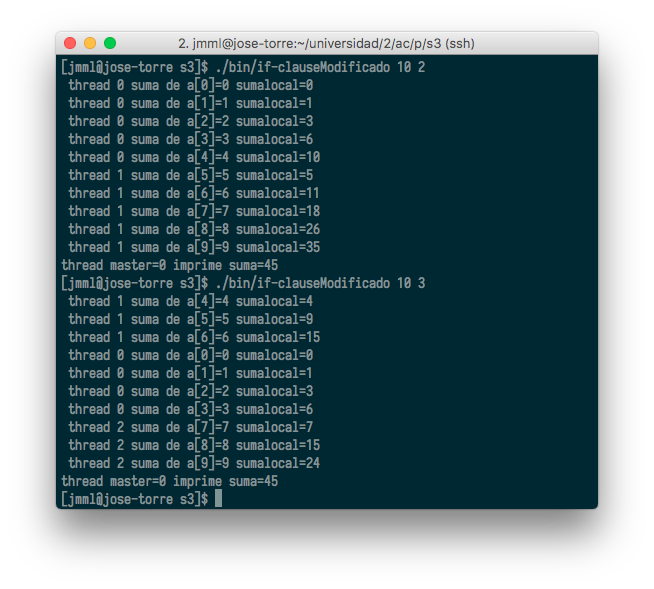
\includegraphics[width=0.8\linewidth]{./img/11.png}
    \label{fig:}
\end{figure}

\emph{Respuesta.} La captura de pantalla ilustra que esta cláusula permite limitar el número de \textit{threads} que utiliza el programa. Efectivamente, en la primera ejecución al poner el valor 2 el programa sólo utiliza 2 \textit{threads} (0, 1), y en la segunda, con el valor 3, los \textit{threads} 0, 1 y 2.\\

\global\arrayrulewidth=1pt
\pgfplotstableset{
    empty cells with={--}, % replace empty cells with ’--’
    every head row/.style={after row=\arrayrulecolor{300}\hline},
    every last row/.style={after row=\arrayrulecolor{300}\hline}
}

%2
\begin{ejer}\hfill
    \begin{enumerate}[label=\alph*)]
        \item Rellena la Tabla 1 (se debe poner en la tabla el \textit{id} del thread que ejecuta cada iteración) ejecutando los ejemplos del seminario \texttt{schedule-clause.c}, \texttt{scheduled-clause.c} y \texttt{scheduleg-clause.c} con dos threads (0, 1) y unas entradas de: \begin{itemize}
            \item iteraciones: 16 (0, ..., 15)
            \item chunk: 1, 2 y 4
        \end{itemize}
        \item Rellena otra tabla como la de la figura pero esta vez usando cuatro \textit{threads} (0, 1, 2, 3).
    \end{enumerate}
    Escribe en el cuaderno de prácticas las diferencias en el comportamiento de \texttt{schedule()} con \texttt{static}, \texttt{dynamic} y \texttt{guided}.
\end{ejer}

\begin{figure}[h]
    \caption{Tablas schedule. 1, 2 y 4 representan el tamaño del \emph{chunk}. Se han utilizado dos \textit{threads}}
    \begin{minipage}[t]{.33\linewidth}
        \centering
        \captionof*{table}{ \texttt{schedule-clause.c} }
        \pgfplotstabletypeset[ % local config, applies only for this table
        1000 sep={\,},
        columns/info/.style={
            fixed,fixed zerofill,precision=1,showpos,
            column type=r,
        },
        %every head row/.style={before row=\caption{Test}},
        ]
        {./dat/schedule-clause1.dat}
    \end{minipage}
    \begin{minipage}[t]{.33\linewidth}
        \centering
        \captionof*{table}{ \texttt{scheduled-clause.c} }
        \pgfplotstabletypeset[ % local config, applies only for this table
        1000 sep={\,},
        columns/info/.style={
            fixed,fixed zerofill,precision=1,showpos,
            column type=r,
        },
        %every head row/.style={before row=\caption{Test}},
        ]
        {./dat/scheduled-clause1.dat}
    \end{minipage}
    \begin{minipage}[t]{.33\linewidth}
        \centering
        \captionof*{table}{ \texttt{scheduleg-clause.c} }

        \pgfplotstabletypeset[ % local config, applies only for this table
        1000 sep={\,},
        columns/info/.style={
            fixed,fixed zerofill,precision=1,showpos,
            column type=r,
        },
        %every head row/.style={before row=\caption{Test}},
        ]
        {./dat/scheduleg-clause1.dat}
    \end{minipage}
\end{figure}

\begin{figure}[H]
    \caption{Tablas schedule. 1, 2 y 4 representan el tamaño del \emph{chunk}. Se han utilizado cuatro \textit{threads}}
    \begin{minipage}[t]{.33\linewidth}
        \centering
        \captionof*{table}{ \texttt{schedule-clause.c} }
        \pgfplotstabletypeset[ % local config, applies only for this table
        1000 sep={\,},
        columns/info/.style={
            fixed,fixed zerofill,precision=1,showpos,
            column type=r,<D-+>
        },
        %every head row/.style={before row=\caption{Test}},
        ]
        {./dat/schedule-clause2.dat}
    \end{minipage}
    \begin{minipage}[t]{.33\linewidth}
        \centering
        \captionof*{table}{ \texttt{scheduled-clause.c} }
        \pgfplotstabletypeset[ % local config, applies only for this table
        1000 sep={\,},
        columns/info/.style={
            fixed,fixed zerofill,precision=1,showpos,
            column type=r,
        },
        %every head row/.style={before row=\caption{Test}},
        ]
        {./dat/scheduled-clause2.dat}
    \end{minipage}
    \begin{minipage}[t]{.33\linewidth}
        \centering
        \captionof*{table}{ \texttt{scheduleg-clause.c} }

        \pgfplotstabletypeset[ % local config, applies only for this table
        1000 sep={\,},
        columns/info/.style={
            fixed,fixed zerofill,precision=1,showpos,
            column type=r,
        },
        %every head row/.style={before row=\caption{Test}},
        ]
        {./dat/scheduleg-clause2.dat}
    \end{minipage}
\end{figure}

\emph{Respuesta:} Las diferencias son las siguientes: \begin{itemize}
    \item \texttt{static} asigna los \textit{threads} correspondientes a cada iteración mediante un algoritmo \textit{round-robin}. La ventaja que tiene es que si se tienen dos cargas de trabajo que se distribuyen entre el mismo número de \textit{threads} siempre le corresponderá el mismo rango de iteraciones a cada \textit{thread}. Los bucles se dividen en \textit{chunks} del mismo tamaño o similar en el caso de que haya un resto al dividir.
    \item \texttt{dynamic} asigna los \textit{threads} por orden de llegada. De nuevo, los bucles se dividen en \textit{chunks} del mismo tamaño.
    \item \texttt{guided} es similar a \texttt{dynamic} pero el \textit{chunk} va reduciendo su tamaño en cada asignación. El parámetro \texttt{chunk} indica el tamaño mínimo que puede tener.
\end{itemize}

\begin{ejer}
    Añade al programa \texttt{scheduled-clause.c} lo necesario para que imprima el valor de las variables de control \texttt{dyn-var}, \texttt{nthreads-var}, \texttt{thread-limit-var} y \texttt{run-sched-var} dentro (debe imprimir sólo un thread) y fuera de la región paralela. Realiza varias ejecuciones usando variables de entorno para modificar estas variables de control antes de la ejecución. Incorpora en tu cuaderno de prácticas volcados de pantalla de estas ejecuciones. ¿Se imprimen valores distintos dentro y fuera de la región paralela?
\end{ejer}

\lstinputlisting[caption=scheduled-clauseModificado.c, language=C]{./src/scheduled-clauseModificado.c}

\begin{figure}[H]
    \centering
    \caption{Sin modificar variables de entorno}
    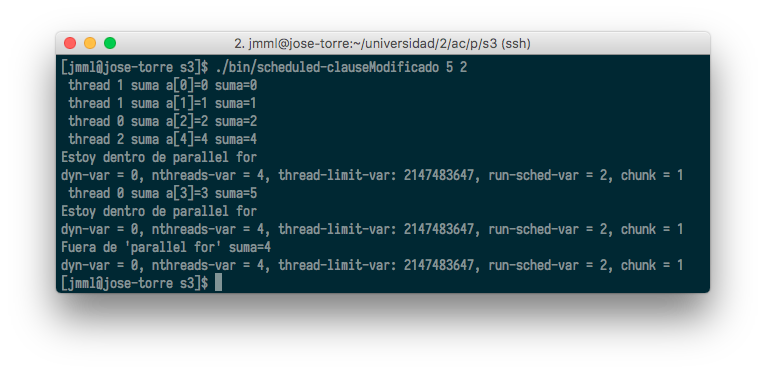
\includegraphics[width=0.9\linewidth]{./img/31.png}
    \label{fig:}
\end{figure}

\begin{figure}[H]
    \centering
    \caption{Modificando \texttt{OMP\_NUM\_THREADS}}
    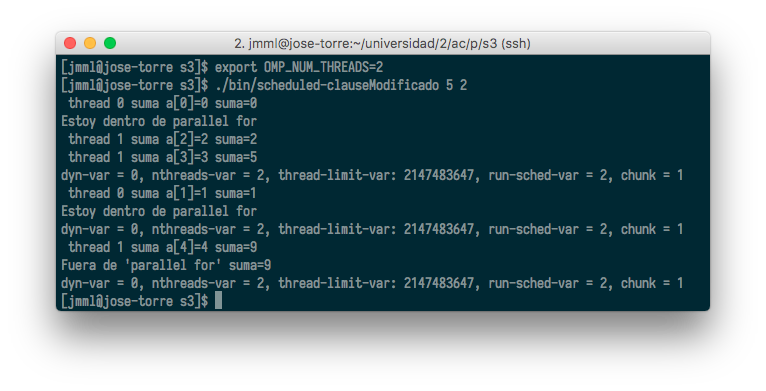
\includegraphics[width=0.9\linewidth]{./img/32.png}
    \label{fig:}
\end{figure}

\begin{figure}[H]
    \centering
    \caption{Modificando \texttt{OMP\_THREAD\_LIMIT}}
    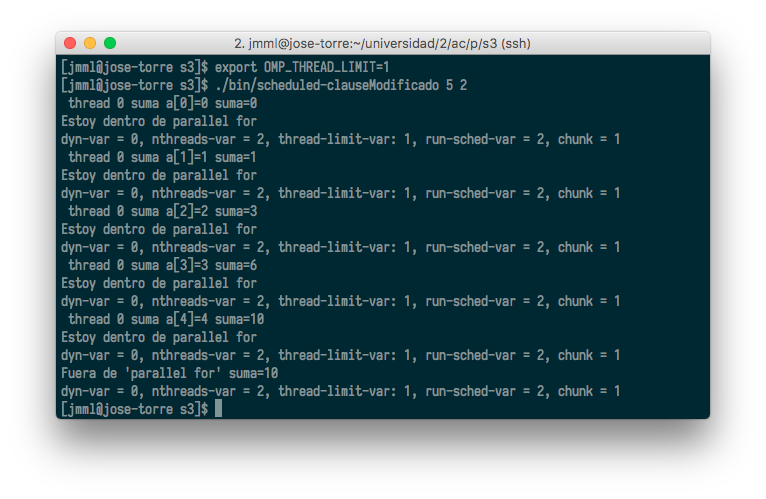
\includegraphics[width=0.9\linewidth]{./img/33.png}
    \label{fig:}
\end{figure}

\emph{Respuesta:} Como se puede observar, los resultados son los mismos dentro de la región paralela y fuera de la misma.

\begin{ejer}
    Usa en el ejemplo anterior las funciones \texttt{omp\_get\_num\_threads()}, \\ \texttt{omp\_get\_num\_procs()} y \texttt{omp\_in\_parallel()} dentro y fuera de la región paralela. Imprime los valores que obtienen estas funciones dentro (lo debe imprimir sólo uno de los threads) y fuera de la región paralela. Incorpora en tu cuaderno de prácticas volcados de pantalla con los resultados de ejecución obtenidos. Indica en qué funciones se obtienen valores distintos dentro y fuera de la región paralela.
\end{ejer}

\lstinputlisting[caption=scheduled-clauseModificado4.c, language=C]{./src/scheduled-clauseModificado4.c}

\begin{figure}[H]
    \centering
    \caption{Valores de las funciones dentro y fuera}
    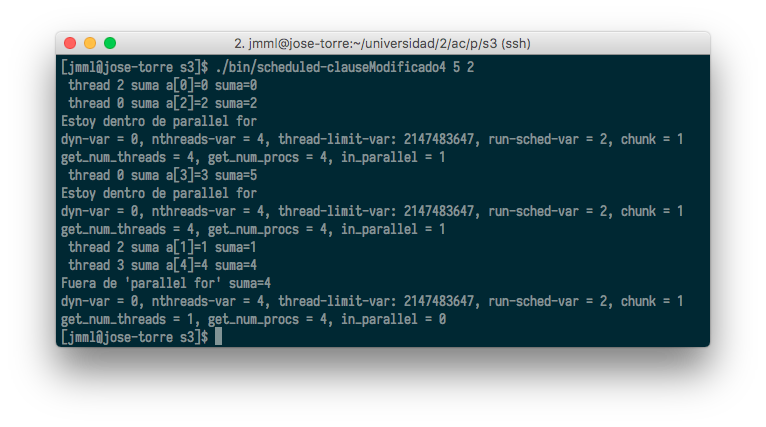
\includegraphics[width=0.9\linewidth]{./img/41.png}
    \label{fig:}
\end{figure}

\emph{Respuesta:} Las variables que cambian son \texttt{get\_num\_threads} e \texttt{in\_parallel}. Era de esperar ya que al salir de la región paralela el número de \textit{threads} será 1 y el indicador, 0.

\begin{ejer}
    Añade al programa \texttt{scheduled-clause.c} lo necesario para modificar las variables de control \texttt{dyn-var}, \texttt{nthreads-var} y \texttt{run-sched-var} y para poder imprimir el valor de estas variables antes y después de dicha modificación. Incorpora en tu cuaderno de prácticas volcados de pantalla con los resultados de ejecución obtenidos.
\end{ejer}

\lstinputlisting[caption=scheduled-clauseModificado5.c, language=C]{./src/scheduled-clauseModificado5.c}

\begin{figure}[H]
    \centering
    \caption{Valores de las variables}
    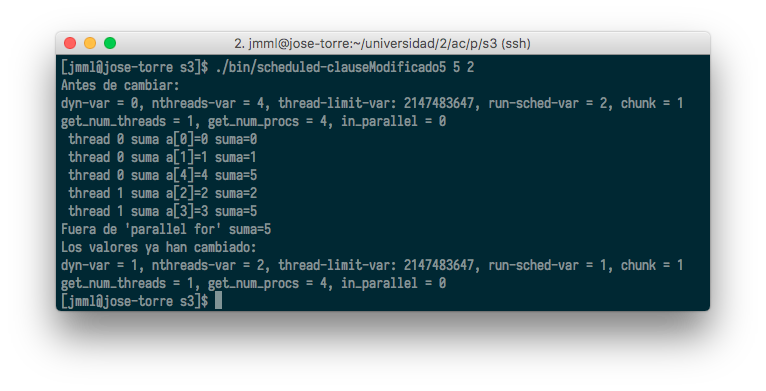
\includegraphics[width=0.9\linewidth]{./img/51.png}
    \label{fig:}
\end{figure}

\section*{Resto de ejercicios}
\label{sec:resto_de_ejercicios}

\begin{ejer}
    Implementa un programa secuencial en C que multiplique una matriz triangular por un vector (use variables dinámicas). Compara el orden de complejidad del código que has implementado con el código que implementaste para el producto matriz por vector.
    
    \hfill\\
    \textit{Notas.} \small \begin{itemize}
        \item El número de filas/columnas debe ser un argumento de entrada
        \item Se debe inicializar las matrices antes del cálculo
        \item Se debe imprimir siempre la primera y última componente del resultado antes de que termine el programa.
    \end{itemize} 
\end{ejer}

\lstinputlisting[caption=pmtv-secuencial.c, language=C]{./src/pmtv-secuencial.c}

\begin{figure}[H]
    \centering
        \caption{Resultados para matriz $10 \times 10$}
    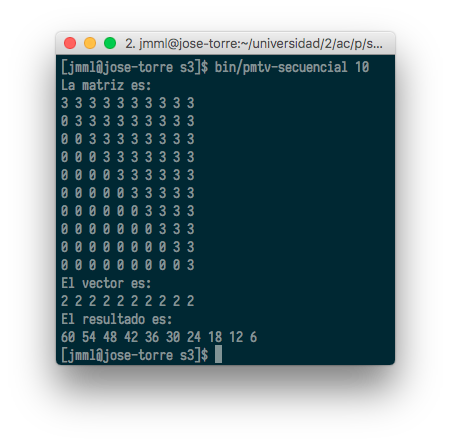
\includegraphics[width=0.6\linewidth]{./img/61.png}
    \label{fig:}
\end{figure}

\begin{figure}[H]
    \centering
    \caption{Resultados para matriz $20 \times 20$}
    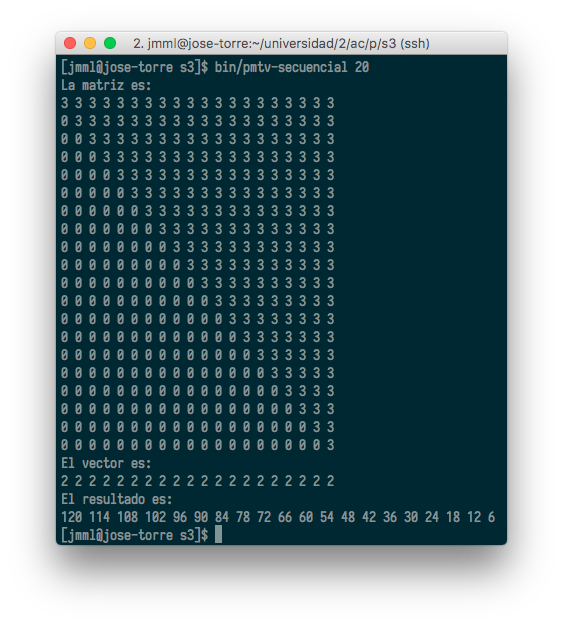
\includegraphics[width=0.7\linewidth]{./img/62.png}
    \label{fig:}
\end{figure}

\emph{Respuesta:} El orden de complejidad de ambos algoritmos es $O(n^2)$.

\begin{lstlisting}[language=C, caption=Producto de matriz por vector]
    for (i = 0; i < N; i++)
        for(j = 0; j < N; j++)
            v2[i] += m[i][j] * v1[j];
\end{lstlisting}

Tenemos dos bucles de tamaño $N$ que realizan una operación $O(1)$. Luego el orden de complejidad es $O(1) \cdot N \cdot N = O(N^2)$.

\begin{lstlisting}[language=C, caption=Producto de matriz triangular por vector]
for (i = 0; i < N; ++i)
        for (j = i; j < N; ++j)
            res[i] += matriz[i][j] * vector[j];
\end{lstlisting}

De nuevo tenemos dos bucles, pero en este caso uno es de tamaño $N$ y el otro de tamaño $\frac{N}{2}$ dado que la matriz es triangular. Aún así el orden de complejidad es $O(1) \cdot N \cdot \frac{N}{2} = O(N^2)$.

\begin{ejer}
    Implementa en paralelo la multiplicación de una matriz triangular por un vector a partir del código secuencial realizado para el ejercicio anterior utilizando la directiva \texttt{for} de OpenMP. El código debe repartir entre los threads las iteraciones del bucle que recorre las filas. Dibuja en el cuaderno de prácticas la descomposición de dominio utilizada (Lección 4/Tema 2) en el código paralelo implementado para asignar tareas a los threads (Lección 5/Tema 2). Añade lo necesario para que el usuario pueda fijar la planificación de tareas usando la variable de entorno \texttt{OMP\_SCHEDULE}. Obtén en atcgrid los tiempos de ejecución del código paralelo (usando, como siempre, -O2 al compilar) que multiplica una matriz triangular por un vector con las alternativas de planificación \texttt{static,} \texttt{dynamic} y \texttt{guided} para chunk de 1, 64 y el chunk por defecto para la alternativa. Usa un tamaño de vector N múltiplo del número de cores y de 64 que no sea inferior a 15360. El número de threads en las ejecuciones debe coincidir con el número de cores. Rellenar la Tabla 3 dos veces con los tiempos obtenidos. Representa el tiempo para \texttt{static}, \texttt{dynamic} y \texttt{guided} en función del tamaño del chunk en una gráfica. ¿Qué alternativa ofrece mejores prestaciones? Razona por qué. Incluye los scripts utilizado en el cuaderno de prácticas.
    
    \hfill\\
    \textit{Nota:} Nunca ejecutes en atcgrid código que imprima todos los componentes del resultado.
    
    Contesta a las siguientes preguntas:

    \begin{enumerate}[label=\alph*)]
        \item ¿Qué valor por defecto usa OpenMP para \texttt{chunk} con \texttt{static}, \texttt{dynamic} y \texttt{guided}? Indica qué ha hecho para obtener este valor por defecto para cada alternativa.
        \item ¿Qué número de operaciones de multiplicación y suma realizan cada uno de los threads en la asignación \texttt{static} para cada uno de los \texttt{chunks}?
        \item Con la asignación \texttt{dynamic} y \texttt{guided}, ¿qué crees que debe ocurrir con el número de operaciones de multiplicación y suma que realizan cada uno de los threads?
    \end{enumerate}
\end{ejer}

%TODO Descomposición de dominio
%\textit{Descomposición de dominio}: Dado que utilizamos \texttt{private(j)}, a cada \textit{thread} le corresponde una fila de la matriz. 

%\begin{figure}[H]
%    \centering
%    \begin{tikzpicture}
%    \tkzDefPoint(0,0){T4}
%    \tkzDefPoint(2,0){p41}
%    \tkzDefPoint(3,0){p42}
%    \tkzDefPoint(4,0){p43}
%    \tkzDefPoint(5,0){p44}
%    \tkzDefPoint(1.5,0.5){r41}
%    \tkzDefPoint(1.5,-0.5){r42}
%    \tkzDefPoint(5.5,0.5){r43}
%    \tkzDefPoint(5.5,-0.5){r44}
    
%    \tkzDrawPolygon[color=500,fill=50](r41,r42,r44,r43)
%    \tkzLabelPoints[above=-1em](T4, p41, p42, p43, p44)

%    \tkzDefPoint(0,1.5){T3}
%    \tkzDefPoint(2,1.5){p31}
%    \tkzDefPoint(3,1.5){p32}
%    \tkzDefPoint(4,1.5){p33}
%    \tkzDefPoint(5,1.5){p34}
%    \tkzDefPoint(1.5,2){r31}
%    \tkzDefPoint(1.5,1){r32}
%    \tkzDefPoint(5.5,2){r33}
%    \tkzDefPoint(5.5,1){r34}
%    
%    \tkzDrawPolygon[color=500,fill=50](r31,r32,r34,r33)
%    \tkzLabelPoints[above=-1em](T3, p31, p32, p33, p34)
%
%    \tkzDefPoint(0,3){T2}
%    \tkzDefPoint(2,3){p21}
%    \tkzDefPoint(3,3){p22}
%    \tkzDefPoint(4,3){p23}
%    \tkzDefPoint(5,3){p24}
%    \tkzDefPoint(1.5,3.5){r21}
%    \tkzDefPoint(1.5,2.5){r22}
%    \tkzDefPoint(5.5,3.5){r23}
%    \tkzDefPoint(5.5,2.5){r24}
%    
%    \tkzDrawPolygon[color=500,fill=50](r21,r22,r24,r23)
%    \tkzLabelPoints[above=-1em](T2, p21, p22, p23, p24)
%
%    \tkzDefPoint(0,4.5){T1}
%    \tkzDefPoint(2,4.5){p11}
%    \tkzDefPoint(3,4.5){p12}
%    \tkzDefPoint(4,4.5){p13}
%    \tkzDefPoint(5,4.5){p14}
%    \tkzDefPoint(1.5,5){r11}
%    \tkzDefPoint(1.5,4){r12}
%    \tkzDefPoint(5.5,5){r13}
%    \tkzDefPoint(5.5,4){r14}
%    
%    \tkzDrawPolygon[color=500,fill=50](r11,r12,r14,r13)
%    \tkzLabelPoints[above=-1em](T1, p11, p12, p13, p14)
%
%    \tkzDefPoint(3.5,5.5){mtext}
%    \tkzLabelPoint[above=-1em](mtext){Matriz}
%
%    %\tkzDefPoint(7,4.5){T1}
%    \tkzDefPoint(8,4.5){v1}
%    \tkzDefPoint(8,3){v2}
%    \tkzDefPoint(8,1.5){v3}
%    \tkzDefPoint(8,0){v4}
%    \tkzDefPoint(7.5,5){rv1}
%    \tkzDefPoint(7.5,-.5){rv2}
%    \tkzDefPoint(8.5,5){rv3}
%    \tkzDefPoint(8.5,-.5){rv4}
%    
%    \tkzDrawPolygon[color=500,fill=50](rv1, rv2, rv4, rv3)
%    \tkzLabelPoints[above=-1em](v1, v2, v3, v4)
%
%    \tkzDefPoint(8,5.5){vtext}
%    \tkzLabelPoint[above=-1em](vtext){Vector}
%
%
%\end{tikzpicture}
%    \label{fig:}
%\end{figure}

\lstinputlisting[caption=pmtv-OpenMP.c, language=C]{./src/pmtv-OpenMP.c}

\begin{figure}[H]
    \centering
        \caption{Resultados para matriz $10 \times 10$}
    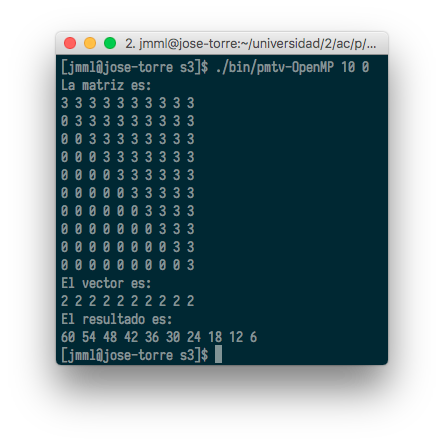
\includegraphics[width=0.6\linewidth]{./img/71.png}
    \label{fig:}
\end{figure}

\begin{figure}[H]
    \centering
    \caption{Resultados para matriz $20 \times 20$}
    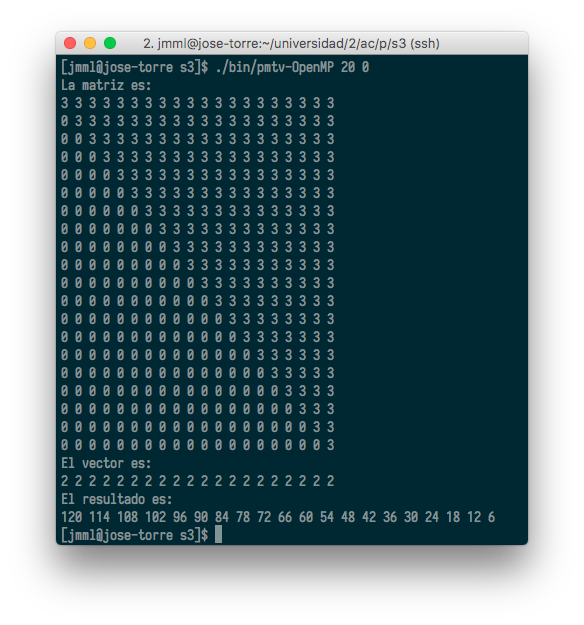
\includegraphics[width=0.7\linewidth]{./img/72.png}
    \label{fig:}
\end{figure}

\lstinputlisting[caption=pmtv-OpenMP-atcgrid.sh, language=Bash]{./pmtv-OpenMP-atcgrid.sh}

% Aquí la tabla 

\begin{figure}[H]
    \caption{Tiempos de ejecución (primera vez) de la versión paralela del producto de una matriz triangular por un vector $r$  para vectores de tamaño $N = 12$ threads}
        \centering
        \pgfplotstabletypeset[ % local config, applies only for this table
        1000 sep={\,},
        columns/Chunk/.style={string type,column type=c},
        columns/info/.style={
            fixed,fixed zerofill,precision=1,showpos,
            column type=r,
        },
        columns/Chunk/.style={string type,column type=c},
        columns/Static/.style={
            fixed,fixed zerofill,precision=3,
            column type=r,
            postproc cell content/.append style={
                /pgfplots/table/@cell content/.add={}{s},
            }
        },
        columns/Dynamic/.style={
            fixed,fixed zerofill,precision=3,
            column type=r,
            postproc cell content/.append style={
                /pgfplots/table/@cell content/.add={}{s},
            }
        },
        columns/Guided/.style={
            fixed,fixed zerofill,precision=3,
            column type=r,
            postproc cell content/.append style={
                /pgfplots/table/@cell content/.add={}{s},
            }
        },
        ]
        {./dat/pmtv-OpenMP1.dat}
\end{figure}

\begin{figure}[H]
    \caption{Tiempos de ejecución (segunda vez) de la versión paralela del producto de una matriz triangular por un vector $r$  para vectores de tamaño $N = 12$ threads}
        \centering
        \pgfplotstabletypeset[ % local config, applies only for this table
        1000 sep={\,},
        columns/info/.style={
            fixed,fixed zerofill,precision=1,showpos,
            column type=r,
        },
        columns/Chunk/.style={string type,column type=c},
        columns/Static/.style={
            fixed,fixed zerofill,precision=3,
            column type=r,
            postproc cell content/.append style={
                /pgfplots/table/@cell content/.add={}{s},
            }
        },
        columns/Dynamic/.style={
            fixed,fixed zerofill,precision=3,
            column type=r,
            postproc cell content/.append style={
                /pgfplots/table/@cell content/.add={}{s},
            }
        },
        columns/Guided/.style={
            fixed,fixed zerofill,precision=3,
            column type=r,
            postproc cell content/.append style={
                /pgfplots/table/@cell content/.add={}{s},
            }
        },
        col sep = tab,
        ]
        {./dat/pmtv-OpenMP2.dat}
\end{figure}


% Aquí la gráfica

\begin{minipage}[t]{.5\linewidth}
    \pgfplotstableread{./dat/pmtv-OpenMP1.dat}{\pmtvOpenMPuno}
    \begin{figure}[H]
        \caption{Primera ejecución}
        \begin{tikzpicture}[scale=.9]
            \begin{axis}[
                xlabel=Chunk,
                ylabel=Tiempo (s),
                xtick=data,
                xticklabels from table={./dat/pmtv-OpenMP1.dat}{Chunk},
                yticklabel style={/pgf/number format/fixed},
                legend pos=north west,
                ]
                \addplot [500,very thick] table [x expr=\coordindex, y={Static}] {\pmtvOpenMPuno};
                \addlegendentry{Static}
                \addplot [700,very thick] table [x expr=\coordindex, y={Dynamic}] {\pmtvOpenMPuno};
                \addlegendentry{Dynamic}
                \addplot [900,very thick] table [x expr=\coordindex, y={Guided}] {\pmtvOpenMPuno};
                \addlegendentry{Guided}
            \end{axis}
        \end{tikzpicture}
    \end{figure}
\end{minipage}\hfill
\begin{minipage}[t]{.5\linewidth}
    \pgfplotstableread[col sep = tab]{./dat/pmtv-OpenMP2.dat}{\pmtvOpenMPuno}
    \begin{figure}[H]
        \caption{Segunda ejecución}
        \begin{tikzpicture}[scale=.9]
            \begin{axis}[,
                xlabel=Chunk,
                ylabel=Tiempo (s),
                xtick=data,
                xticklabels from table={./dat/pmtv-OpenMP2.dat}{Chunk},
                yticklabel style={/pgf/number format/fixed},
                legend pos=north east,
                ]
                \addplot [500,very thick] table [x expr=\coordindex, y={Static}] {\pmtvOpenMPuno};
                \addlegendentry{Static}
                \addplot [700,very thick] table [x expr=\coordindex, y={Dynamic}] {\pmtvOpenMPuno};
                \addlegendentry{Dynamic}
                \addplot [900,very thick] table [x expr=\coordindex, y={Guided}] {\pmtvOpenMPuno};
                \addlegendentry{Guided}
            \end{axis}
        \end{tikzpicture}
    \end{figure}
\end{minipage}


\emph{Respuestas:}

\begin{enumerate}[label=\alph*)]
        \item El valor por defecto de \texttt{chunk} en \texttt{static} es $  \frac{número \ de \ iteraciones}{número \ de \ threads}$, el de \texttt{dynamic} es 1 y el de \texttt{guided}, de nuevo $ \frac{número \ de \ iteraciones}{número \ de \ threads}$. La información la he obtenido en la documentación de OpenMP.
        \item Para el \textit{chunk} por defecto, cada thread hace $ \frac{N}{12} \cdot 2$ (2 es el número de sumas y multiplicaciones por iteración). Con el \texttt{chunk} = 1, de nuevo $ \frac{N}{12} \cdot 2$ operaciones y con \texttt{chunk} = 64, realizará como mínimo $\frac{N}{64} \cdot \frac{1}{12} \cdot 2$ operaciones. En este último caso lo que se ha hecho es dividir $\frac{número \ de \ iteraciones}{tamaño \ de \ \textit{chunk}}$ para saber cuántos \textit{chunks} habrá en total. Entonces como mínimo, cada \textit{thread} ejecutará $ \frac{número \ de \ chunks}{número \ de \ threads}$. Los \textit{chunks} sobrantes se repartirán entre el total de \textit{threads}.
        \item Variará en distintas ejecuciones ya que no están asignados de forma fija y depende del tiempo que tarde cada \textit{thread} en realizar las operaciones.
    \end{enumerate}

A la vista de los datos la alternativa que ofrece mejores prestaciones es \texttt{dynamic}. Puede deberse al hecho de que a cada \textit{thread} se le asigna una iteración en cuanto acaba la que tenía asignada en lugar de tenerlas asignadas desde un principio. De esta forma, si algún \textit{thread} acaba más rápido que otro, puede pasar a la siguiente iteración.


\begin{ejer}
    Implementa un programa secuencial en C que calcule la multiplicación de matrices cuadradas, B y C: $$ A = B \cdot C; \ A(i,j) = \sum_{k=0}^{N-1} B(i,k) \cdot C(k,j), \ i,j=0, \hdots N-1$$

    \hfill\\
    \textit{Notas.} \small \begin{itemize}
        \item El número de filas/columnas debe ser un argumento de entrada.
        \item Se debe inicializar las matrices antes del cálculo.
        \item Se debe imprimir siempre las camponentes $(0,0)$ y $(N-1, N-1)$ del resultado antes de que termine el programa.
    \end{itemize} 
\end{ejer}

\lstinputlisting[caption=pmm-secuencial.c, language=C]{./src/pmm-secuencial.c}

\begin{figure}[H]
    \centering
    \caption{Resultados para varios tamaños}
    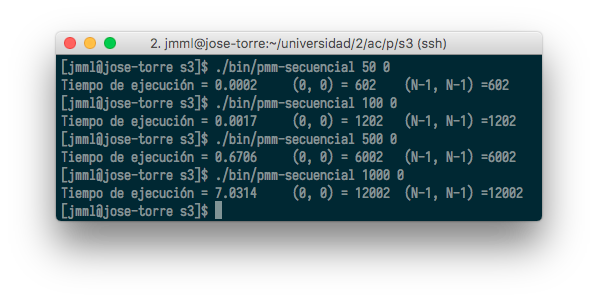
\includegraphics[width=0.8\linewidth]{./img/81.png}
    \label{fig:}
\end{figure}

\begin{ejer}
    Implementa en paralelo la multiplicación de matrices cuadradas con OpenMP a partir del código escrito en el ejercicio anterior. Usa las directivas, las cláusulas y las funciones de entorno que consideres oportunas. Se debe paralelizar también la inicialización de las matrices. Dibuja en su cuaderno de prácticas la descomposición de dominio que ha utilizado en el código paralelo implementado para asignar tareas a los threads (Lección 4/Tema 2,Lección 5/Tema 2).
\end{ejer}

%\textit{Descomposición de dominio}:
%TODO: Descomposición de dominio

\lstinputlisting[caption=pmm-OpenMP.c, language=C]{./src/pmm-OpenMP.c}

\begin{figure}[H]
    \centering
    \caption{Resultados para varios tamaños}
    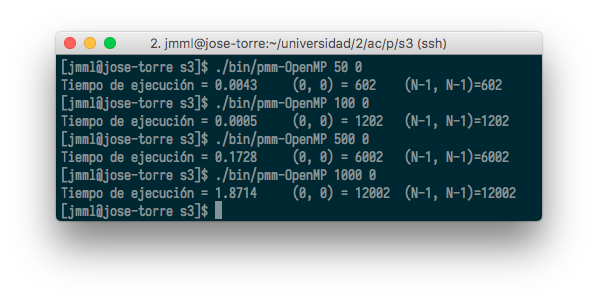
\includegraphics[width=0.8\linewidth]{./img/91.png}
    \label{fig:}
\end{figure}

\begin{ejer}
    Haz un estudio de escalabilidad (ganancia en velocidad en función del número de cores) en atcgrid y en el PC local del código paralelo implementado para dos tamaños de las matrices. Debes recordar usar –O2 al compilar. Presenta los resultados del estudio en tablas de valores y en gráficas. Escoge los tamaños de manera que se observen diferentes curvas de escalabilidad en las gráficas que entregues en tu cuaderno de prácticas (prueba con valores de N entre 100 y 1500). Consulta la Lección 6/Tema 2. Incluye los scripts utilizado en el cuaderno de prácticas. 
    
    \hfill\\
    \textit{Nota:} \small Nunca ejecute en atcgrid código que imprima todos los componentes del resultado.
    
\end{ejer}

% Tablas

\begin{minipage}[t]{.5\linewidth}
\begin{figure}[H]
    \caption{Estudio de escalabilidad en el PC local}
        \centering
        \pgfplotstabletypeset[ % local config, applies only for this table
        columns/Elementos/.style={
            1000 sep={}
        },
        columns/Secuencial/.style={
            fixed,fixed zerofill,precision=3,
            column type=r,
            postproc cell content/.append style={
                /pgfplots/table/@cell content/.add={}{s},
            }
        },
        columns/2 threads/.style={
            fixed,fixed zerofill,precision=3,
            column type=r,
            postproc cell content/.append style={
                /pgfplots/table/@cell content/.add={}{s},
            }
        },
        columns/4 threads/.style={
            fixed,fixed zerofill,precision=3,
            column type=r,
            postproc cell content/.append style={
                /pgfplots/table/@cell content/.add={}{s},
            }
        },
        col sep = tab,
        ]
        {./dat/pmm-escalabilidad-pclocal.dat}
\end{figure}
\end{minipage}\hfill
\begin{minipage}[t]{.5\linewidth}
\begin{figure}[H]
    \caption{Estudio de escalabilidad en atcgrid}
        \centering
        \pgfplotstabletypeset[ % local config, applies only for this table
        columns/Secuencial/.style={
            fixed,fixed zerofill,precision=3,
            column type=r,
            postproc cell content/.append style={
                /pgfplots/table/@cell content/.add={}{s},
            }
        },
        columns/2 threads/.style={
            fixed,fixed zerofill,precision=3,
            column type=r,
            postproc cell content/.append style={
                /pgfplots/table/@cell content/.add={}{s},
            }
        },
        columns/4 threads/.style={
            fixed,fixed zerofill,precision=3,
            column type=r,
            postproc cell content/.append style={
                /pgfplots/table/@cell content/.add={}{s},
            }
        },
        col sep = tab,
        ]
        {./dat/pmm-escalabilidad-atcgrid.dat}
\end{figure}
\end{minipage}

\begin{minipage}[t]{.5\linewidth}
\pgfplotstableread[col sep = tab]{./dat/pmm-escalabilidad-pclocal.dat}{\pmmpclocal}
    \begin{figure}[H]
        \centering
        \caption{Estudio de escalabilidad en el PC local}
        \begin{tikzpicture}[scale=.9]
            \begin{axis}[
                xlabel=Elementos,
                ylabel=Tiempo (s),
                %xtick=data,
                %xticklabels from table={./dat/pmtv-OpenMP2.dat}{Chunk},
                yticklabel style={/pgf/number format/fixed},
                legend pos=north west,
                max space between ticks=50pt,
                ]
                \addplot [500,very thick] table [x={Elementos}, y={Secuencial}] {\pmmpclocal};
                \addlegendentry{Secuencial}
                \addplot [700,very thick] table [x={Elementos}, y={2 threads}] {\pmmpclocal};
                \addlegendentry{2 threads}
                \addplot [900,very thick] table [x={Elementos}, y={4 threads}] {\pmmpclocal};
                \addlegendentry{4 threads}
            \end{axis}
        \end{tikzpicture}
    \end{figure}
\end{minipage}\hfill
\begin{minipage}[t]{.5\linewidth}
\pgfplotstableread[col sep = tab]{./dat/pmm-escalabilidad-atcgrid.dat}{\pmmatcgrid}
    \begin{figure}[H]
        \centering
        \caption{Estudio de escalabilidad en atcgrid}
        \begin{tikzpicture}[scale=.9]
            \begin{axis}[
                xlabel=Elementos,
                ylabel=Tiempo (s),
                %xtick=data,
                %xticklabels from table={./dat/pmtv-OpenMP2.dat}{Chunk},
                yticklabel style={/pgf/number format/fixed},
                legend pos=north west,
                max space between ticks=50pt,
                ]
                \addplot [500,very thick] table [x={Elementos}, y={Secuencial}] {\pmmatcgrid};
                \addlegendentry{Secuencial}
                \addplot [700,very thick] table [x={Elementos}, y={2 threads}] {\pmmatcgrid};
                \addlegendentry{2 threads}
                \addplot [900,very thick] table [x={Elementos}, y={4 threads}] {\pmmatcgrid};
                \addlegendentry{4 threads}
            \end{axis}
        \end{tikzpicture}
    \end{figure}
\end{minipage}

% Gráficas

\lstinputlisting[caption=pmm-OpenMP-atcgrid.sh, language=Bash]{./pmm-escalabilidad-atcgrid.sh}
\lstinputlisting[caption=pmm-OpenMP-pclocal.sh, language=Bash]{./pmm-escalabilidad-pclocal.sh}


\end{document}
